\documentclass[a4paper, twocolumn]{article}
\usepackage{CJKutf8}
\usepackage[sc]{mathpazo} % Use the Palatino font
\usepackage[T1]{fontenc} % Use 8-bit encoding that has 256 glyphs
\linespread{1.2} % Line spacing - Palatino needs more space between lines
\usepackage{microtype} % Slightly tweak font spacing for aesthetics

\usepackage[english]{babel} % Language hyphenation and typographical rules

\usepackage[hmarginratio=1:1,top=32mm,left=20mm,right=20mm,columnsep=20pt]{geometry} % Document margins
\usepackage[hang, small,labelfont=bf,up,textfont=it,up]{caption} % Custom captions under/above floats in tables or figures
%\usepackage{booktabs} % Horizontal rules in tables

\usepackage{lettrine} % The lettrine is the first enlarged letter at the beginning of the text

\usepackage{enumitem} % Customized lists
\setlist[itemize]{noitemsep} % Make itemize lists more compact

\usepackage{abstract} % Allows abstract customization
\renewcommand{\abstractnamefont}{\normalfont\itshape\bfseries} % Set the "Abstract" text to bold
\renewcommand{\abstracttextfont}{\normalfont} % Set the abstract itself to small italic text

\usepackage{titlesec} % Allows customization of titles
\renewcommand\thesection{\Roman{section}} % Roman numerals for the sections
\renewcommand\thesubsection{\roman{subsection}} % roman numerals for subsections
\titleformat{\section}[block]{\large\scshape\centering}{\thesection.}{1em}{} % Change the look of the section titles
\titleformat{\subsection}[block]{\large}{\thesubsection.}{1em}{} % Change the look of the section titles

\usepackage{fancyhdr} % Headers and footers
\pagestyle{fancy} % All pages have headers and footers
\fancyhead{} % Blank out the default header
\fancyfoot{} % Blank out the default footer
\fancyhead[C]{
	\begin{CJK}{UTF8}{gbsn}
	《计算机图形学》课程 论文翻译
	\end{CJK}}
\fancyfoot[RO,LE]{\thepage} % Custom footer text
\usepackage{titling} % Customizing the title section

\usepackage{hyperref} % For hyperlinks in the PDF
\hypersetup{hidelinks}

\usepackage{graphicx}
\renewcommand{\normalsize}{\fontsize{10.5pt}{\baselineskip}\selectfont}
%----------------------------------------------------------------------------------------
%	TITLE SECTION
%----------------------------------------------------------------------------------------

\setlength{\droptitle}{-4\baselineskip} % Move the title up

\pretitle{\begin{center}\Huge\bfseries} % Article title formatting
	\posttitle{\end{center}} % Article title closing formatting
\title{计算机图形学中的阴影算法} % Article title
\author{%
	\textsc{Franklin C. Crow} \\[1ex] % Your name
	\normalsize University of Texas at Austin \\ % Your institution
	\normalsize Austin, Texas \\ % Your address 
	\normalsize 原论文链接:\href{http://dl.acm.org/citation.cfm?id=563901}{http://dl.acm.org/citation.cfm?id=563901} \\
	\normalsize 译者:刘阳
}
\date{} % Leave empty to omit a date

%----------------------------------------------------------------------------------------

\begin{document}
\begin{CJK}{UTF8}{gbsn}
	% Print the title
	\maketitle
	
	%----------------------------------------------------------------------------------------
%		ARTICLE CONTENTS
	%----------------------------------------------------------------------------------------
	\section{摘要}

	\section{关键词}
计算机图形学,
隐藏表面移除,
阴影,
描影法,
光栅显示器
	\section{介绍}
现在大多数计算机合成的荫蔽图片有一个主要的缺陷,就是缺少阴影。
尽管当光源和出射点一致时,阴影并不需要。很多早期的实现方式都利用了这一事实。
但是许多对现实感图片有严肃要求的应用(像太空飞船的入轨,飞机的着陆模拟)都要求有阳光照射的图片。
现在已经可以生成包含阴影的很真实的场景图了,但是这些图片的成败依赖于有一个漫射光源的假设,像多云天气时的阳光那种。\\
有些情况下,阴影是很重要的。
一个投射阴影可以让设备的一块重要组件在实际情况下事实上不可见,即使它可以在没有阴影的模拟环境下清晰地显示。
计算机图形学应用到建筑坐落问题,环境影响调查方面时,要求阴影的计算,用来评估空调的需求,或者太阳能的可用性。
更重要的是,阴影提供了有价值的位置信息。一个物体投射到另一个物体上的阴影可以表明空间关系,不然的话,就是模糊的空间关系。
此外,阴影造成了一个有趣的问题。它们应该得到比现在更多的关注。\\
Appel\cite{3}和之后的Bouknight、Kelley\cite{5}展示了对于阴影问题的解决方案,之后在这篇论文中会用对阴影算法分类的方式来讨论这些解决方案。
现在有三类解决方案是可以确认的(也许未来会有还未发现的类别)。
Appel, Bouknight和Kelley提出了一类的解决方案和算法,而另两类提出了但还没有实现。\\
第一类算法,由Appel, Bouknight和Kelley论证,在图片从光栅扫描器生成时检测阴影边界。
通过投影潜在的阴影多边形的边到正在扫描的表面,可以找到投射阴影的边。
由此形成的阴影边之后投影到物体平面。
当穿越一条阴影边时,扫描片段的颜色也会恰当地变换。\\
第二类算法包括两遍隐藏表面算法,或者也许是两种不同算法各只进行一次。
第一遍区分有阴影表面和无阴影表面,然后从和光源一致的角度决定隐藏表面,划分部分有阴影的表面。
接着,有阴影表面的颜色会被修改。
第二遍从观察者的角度来操作这些增强了的数据。\\
第三类阴影算法包括计算一个表面,这个表面包围被物体阴影(它的本影)遮盖的空间体积。
这个本影表面之后被添加到数据中,并且被当作一个不可见的表面。当这个表面被穿透时,会产生穿进或穿出物体阴影的变化。\\
一个对于这三类方案更加完整的解释会随着每个类别建议的实现方式一起给出。
在此之前,会有对光源建模的回顾。
在此之后,是尝试性的对于实践过程中实现这三种途径的难度的比较。
	\section{为光源建模}
通常来说,光源都被建模成点光源或者方向光源。
但是,一个实际的光源有有限的尺寸,一个可能不规则的外形,和一个相对于被展示物体的明确的空间位置。
有限尺寸的光源投射出的阴影包括本影和半影。
本影是指没有从光源接收到光线的阴影空间。
半影是指接收到部分但不是全部光线的阴影空间。
所以对于这样的阴影,都有一个深色的中心区域,环之以边界区域,在边界区域里有从有阴影区域到无阴影区域的平滑过渡。
对于一个不规则形状的光源,可以在本影的外围用一条固定宽度的、线性渐变的条带阴影来估计半影。
我们可以期望半影的计算能够显著增强展示阴影的效果。
所以,我们假设用一个点光源,或者一个无限远离的光源(只用方向描述)。\\
阴影边界通过投射一个物体的轮廓到另一个物体上来决定。
使用的投射类型取决于光源的位置。
用来计算阴影的最简单的光源是无限远离的光源。因为阴影边界通过一次正射投影就可以找到。
另一方面,当光源位于物体空间中时,计算阴影边界的难易程度因位置而不同。
如果光源在视场外,阴影边界的计算采用和图片显示一样的透视投影方式。
但是,当光源在视场内时,必须采用不同的方法。
因为传统的透视变换只对有限的视场准确,所以,要么空间必须被划分成以光源为中心的放射状部分,这样就可以用透视变换,要么就要使用更复杂的三维几何方法。\\
透视变换提供了便利和高效。
但是,下面这种方式也总是可以确定物体空间内的阴影边界。
利用光源的位置和物体轮廓来确定表面,然后计算这个表面和其他物体的相交面。
	\section{第一类:扫描时进行阴影计算}
Appel\cite{2}\cite{3}和之后的Bouknight, Kelley\cite{5}展示了渲染阴影的方法:在扫描图片的时候计算阴影边界。
Appel通过扩展他对于量化不可见性的概念来探测阴影边界。
量化不可见性是一种对于隐藏一个顶点的表面数量的度量。(假设是多边形物体)
这样的话,仅当一条线段上的所有点都是值为零的量化不可见性时,这条线段才是可见的。
Appel的隐藏表面算法可以探测到线段上量化不可见性的变化,然后只画出可见的部分。
这种方法产生一条线段绘制。\\
在扫描时决定阴影表面,同样也可以用来遮盖线段绘制。
通过在相等空间的水平线上和图片平面相交,产生穿过出射点的“切”平面,这样来执行扫描过程。(图 \ref{fig:fig1})
\begin{figure*}[h]
\centering
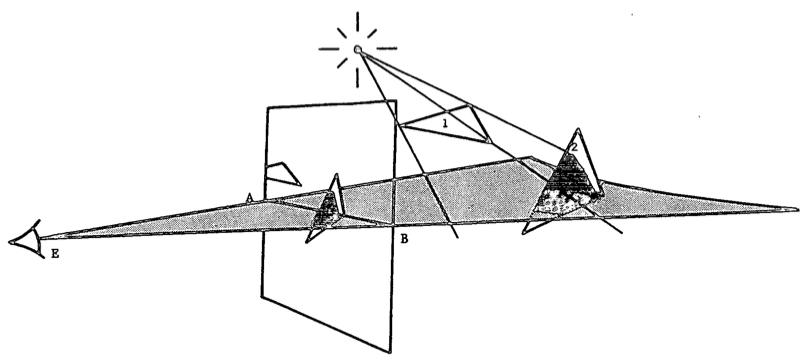
\includegraphics[width=0.9\linewidth]{fig1}
\caption[fig1]{在Appel的算法中,ABE定义了一个“切平面”。多边形1的边投射到多边形2,形成阴影边界,之后投射到图片平面。}
\label{fig:fig1}
\end{figure*}
扫描段的集合由可见线段和切平面的交集决定。
然后对应于光源的量化不可见性(之前已对所有可见顶点算出)会被用来确定那些在阴影中的区段。
更多细节在Appel发表的论文\cite{1}\cite{2}\cite{3}中可见。\\
Bouknight和Kelley开发了一套相似的阴影探测方法\cite{4}\cite{5}。
但是,他们享有一个优势,那就是他们的隐藏表面算法已经基于扫描过程。
通过投射边到正在扫描的表面上,计算出阴影边界,第二次扫描则用来检测这个边界。
主扫描采用图片空间的光栅模式,然后产生第二次扫描,和在物体空间内穿过可见表面的对应路径。
所以,在其他投射到第二次扫描区段的多边形边的地方,就会出现阴影边。\\
一种用来发现所有的可以投射阴影到某个多边形的多边形的步骤被用来减少边投影的计算量。
这个程序将所有的多边形转换成一个伪球形座标空间,而原点在光源处。
多边形之后会测试是否重叠,然后每个多边形都会有一个链接表,使其他可能投射阴影到它上面的多边形可以轻易找到(在图1中,多边形2会链接到多边形1)。
重叠测试的扩展版会引出第二类算法,这将在之后看到。\\
由Bouknight-Kelley提出的典型的通用方法可以解析成两个基本操作:
(1)多边形的阴影优先级顺序 和
(2)计算投射阴影的边界。
值得注意的是,这两个操作相对于显示的隐藏表面算法是独立的,且可以应用到事实上任何基于多边形的算法。\\
可以开发很多基于Bouknight和Kelley的算法的变体。
例如,他们的伪球面重叠测试的算法复杂度是多边形数量的平方。
所以,将可视的物体空间划分成以光源为中心的放射状区域是有利的。
这样就可以将同一个区域内的所有多边形按照阴影优先级顺序排序,而不用参考其他的区域。
确定阴影优先级要求一个特殊的排序方法,例如Newell等人用的方法\cite{9}。
这个算法的行为(同样遵守N方的增长律)在Sutherland等人的论文中有讨论\cite{12}。\\
在有利条件下,分区可以把Bouknight-Kelley(或Newell等人)的N方增长律降低到线性增长律。
分区的增长正比于$ S * (\frac{N}{S})^{2} $,其中S是分区的数量,N是多边形的数量(只要多边形在空间中大体分布保持类似)。
如果增加分区的数量,同时同比例地增加多边形的数量,$ \frac{N}{S} $ 保持不变,那么优先级的步骤就遵守线性增长律。
但是,这个增长速率在受到限制时会变得复杂。当分区足够小时,很大一部分的多边形和分区的边界重叠了,导致多边形的有效数量增加了。
这是因为如果一个多边形横跨了两个分区,那么它必须被两个分区都考虑。
但是,潜在的线性增长速率还是让它成为一个吸引人的方法,不管在这里,还是在通用的分区算法的设计里。\\
第二个基本操作,计算阴影边界,要求一个和裁剪类似的步骤。
正在考虑的多边形必须作为一个窗口,而更高优先级的多边形基于这个窗口进行裁剪。
这个操作的增长速率正比于有阴影多边形的边数和更高优先级多边形的边数的乘积,也是一个N方的增长速率。
但是,分区仍然可以提供一个在有利条件下,总体上线性增长的速率。
(应该注意到,Bouknight和Kelley提出的,在这里使用的链接表在某种程度上是一种优化了的分区。)
有两个因素可以显著减小增长律中的比例常数:
(1)阴影计算只需针对那些可见的多边形进行 和
(2)当一个多边形是完全被阴影遮盖的话,计算可以终止。\\
总结这个部分,应该重新强调的是,在所有阴影算法中,通过仅考虑阴影物体的外围,而不是它的单独的每个多边形,可以减少大量的计算。
这就限制了只要搜索那些产生了可见阴影边界的边。
	\section{第二类:两遍的方式}
对于探测哪些表面是从光源不可见的,和探测哪些表面是从视点不可见的,隐藏表面算法都很容易使用。
但是,为了有用,算法必须生成能被利用的信息,用来在下一遍计算中生成从出射点看到的图片。
这个限制限定了可应用的算法的类别。\\
Sutherland, Sproull 和 Schumaker提出了一种隐藏表面算法,可以分为物体空间算法和图像空间算法\cite{12}。
这种区分是很重要的,因为必须在物体空间里决定阴影的边界,这样生成的信息才能合并进发送到显示算法的数据中。
因为图像空间算法基于显示媒体的有限分辨率,所以用图像空间算法来减轻决定隐藏表面的负担对于这类应用来说是不恰当的。\\
由Sutherland等人描述的算法\cite{12}都严格地在物体空间上操作,都有令人沮丧的增长律(计算复杂度是数据数量的平方)。
此外,当考虑多边形时,它们不是被当作整体,而是被分成了独立对待的面。
为了产生阴影,多边形必须被当作整体,这样它们才能被阴影边界划分开,然后作为更小的多边形返回给数据库,并传递给显示算法。
忽略物体空间算法,剩下了由Newell, Newell和Sancha提出的算法\cite{9}。
这个算法提供了很多有用的技术用来分离多边形和决定重叠部分。
但是最终决定哪个部分的哪个表面是隐藏的,还是通过覆写图像空间来完成的。\\
Sutherland提出了另一种对于此问题更实用的算法\cite{11}。
使用裁剪技术,执行一次二分排序,可以发送多边形和一条线一侧的多边形侧面部分到一条流数据上,而另一侧的侧面部分到另一条流数据上。
当然这种步骤正是决定表面有阴影部分和无阴影部分的划分所需要的。
此外,Sutherland的算法有一个合理的增长速率保证。
因为算法利用对数据的二维二分排序,通过对视场空间的递归划分,可以得到一个$ N\log N $ 的增长律。\\
Sutherland还提出了改进,在子划分的过程中只考虑“轮廓”边。
轮廓边是指分开正面多边形和背面多边形的那些边。
在这些地方,表面曲线会隐藏在自身后面,或者其他表面边缘的边后面。
而这些表面自身没有封闭\cite{1}。
所以,任何区域,只要在单个表面的一组轮廓边的边界内,就可以认为是一个单元,并且假设围起来的表面就是围起来的区域的最前面。\\
Clark提出了一个实现隐藏表面算法的通用模式,用到了对于一种层次化数据描述的递归下降法\cite{7}。
通过将这种方式和Sutherland的轮廓裁剪标注法组合起来,可以保证一个有趣的阴影算法。
如果可以强加一个环境限制:物体一定可以分成线性可分的子物体,和线性可分子物体的组合,那么可以通过以下方式实现一个算法。\\
算法第一步是用和Newell,Newell和Sancha相似的排序技术,来建立一个从正面到背面的待考察表面的优先级顺序。
Clark提出的层次化方法可以叠加到第一顺序的物体或者物体组,然后在这些物体或物体组内再建立一个顺序。
Newell最近建议说,在这里可以应用将物体排序成深度优先顺序的算法\cite{10}。\\
注意到,为了探测阴影,物体的外围可能用来确定一个“印迹”,或者在透视投影下的反窗口。
任何在“印迹”里的东西,并且离光源很远的话,在阴影里都会清除掉。
所以,我们可以交替使用每个顶点子物体的外围来增强一组“印迹”,这样来进行算法。
远离光源,被“印迹”隐藏的表面可以标记为有阴影的。
其他表面将它们外围无阴影的部分添加到“印迹”集合中,然后被裁剪成有阴影和无阴影的部分。\\
通过一个可以提供相邻多边形之间链接的数据结构,找到多边形物体的外围是很容易的。
这种数据结构在\cite{6}\cite{8}中有详细表述。
因为外围是从轮廓边里单独形成的,而且一个顶点表面的所有轮廓边都一定在外围内,所以决定外围的过程包含了找到轮廓边的闭环。\\
轮廓边的串可以很直观地形成。
首先,相对于光源的视角,所有多边形必须被标记为正面,或者背面。
然后,必须检查每个正面多边形的邻居多边形。当找到背面相邻多边形时,它的关联边必须被标记为外围边。
最后,通过使用相邻的正面多边形来搜索连接到一个已知外围顶点的额外外围边,外围边可以连接起来。
对于一个顶点物体,单个的边串可以形成它的外围(图\ref{fig:fig2})。\\
\begin{figure}[h]
\centering
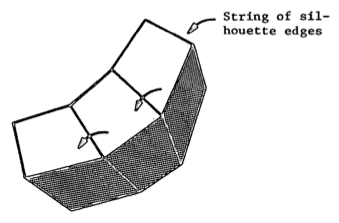
\includegraphics[width=0.9\linewidth]{fig2}
\caption[fig2]{通过搜索相邻正面多边形的轮廓边,可以形成外围边的串。}
\label{fig:fig2}
\end{figure}
通过使用Clark提出的模式,有些物体的外围的计算可以避免。
利用数据的层次性划分(组,物体,子物体),用“界限盒”的测试方法,可以用来决定哪组会从光源视角重叠。
界限盒是用物体顶点的宽高范围决定的(图\ref{fig:fig3})。
\begin{figure}[h]
\centering
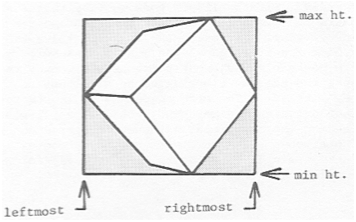
\includegraphics[width=0.9\linewidth]{fig3}
\caption[fig3]{"界限盒“}
\label{fig:fig3}
\end{figure}
任何时候,发现一个物体的界限盒完全在一个更高优先级物体的外围内时,前者物体就在阴影里了。
类似地,如果一个顶点物体(由单个子物体组成)的界限盒没能重叠任何其他物体,那么这个物体显然就不在任何阴影中。
在这种情况下,就没理由要计算外围了。\\
可以用数据的层次结构驱动阴影算法。
所以物体组可以按优先级顺序处理,最近者优先。
在每组物体中,物体会按优先级顺序处理。
在每个物体内,子物体也会按优先级顺序处理。
重叠测试会先确定组间是否有交叉。
如果有,那么界限盒就要传递到下一级更低的层级中。
然后重叠测试会应用到组内的物体间,最终到每个物体的子物体间。
如果一个子物体的界限盒没有和任何层间传递下来的界限盒重叠,那么就可以忽略它了。
否则的话,就要计算它的外围。\\
按照要求计算出高优先级的子物体的外围后,内部物体的阴影边界就可以计算了。
这个计算可以通过在高优先级子物体的外围内裁剪出低优先级子物体的多边形来完成。
如果任何低优先级的子物体是完全阴影覆盖的,那么它就可以标记为完全阴影的,并在之后的重叠测试中忽略掉。
部分阴影覆盖的子物体会被裁剪为有阴影部分和无阴影部分。
然后仅基于无阴影的部分,可以计算出部分的外围。
完全没有被阴影覆盖的子物体仅仅算出了它们的外围而已。\\
当算法按着物体序列的优先级顺序进行运算时,一个顶点印迹的最小集合会构建出来,每个印迹都有与之关联的界限盒。
当处理低优先级的物体时,它们会被更高优先级的印迹裁剪,然后余下的多边形会被用来计算部分外围,结果会加到印迹的集合中。
提前准备将一组印迹吸收进单个印迹中是有用的,以防低优先级的子物体足够大,以至于可以提供一个包裹的外围。
但是,对于这种情况的检查的开销被证实会大于它所带来的益处。\\
当有几组物体重叠时,在所有低优先级组处理完后,很有可能会构建出一个极大的印迹集合。
为了避免过度增长的计算量,印迹的集合和未处理数据应该分区,这样部分分开的区域可以单独处理。
利用界限盒提供的信息,分区会变得简单。
甚至随着印迹集合的增长,重复多分区几次是有利的。
另外,基于低优先级物体的界限盒的分区方式可以将不再需要的印迹丢弃。\\
当然这种方法严重依赖于一个良性条件的环境(顶点子物体)。
并不清楚
(1)该算法是否易于扩展到一般情况 和
(2)数据生成和物体建模技术是否总是可以交付出这样良性条件的数据。\\
一般来讲,上面描述的测试序列会随着包含的物体的数量按平方的复杂度增加开销。
但是,将数据划分成一个层次结构,在印迹数变大时使用分区方式,都会减少必要的测试的数量。
还要再一次指出的是,如果光源在或者靠近出射点的视场时,为了确定阴影,就需要将空间分区,这样透视投影才能派上用场。
这种方法严重依赖于确定正面多边形和背面多边形的难易程度,还依赖于重叠测试。
这两者在一次透视变换后都会变得很容易。\\
一旦阴影多边形确定下来了,任何隐藏表面算法都可以用来从增强的数据中生成出射点图像。
所以,两遍方式的优势就在于,确定阴影的过程和之后图片生成的过程完全独立。
这样阴影处理和图片生成就可以以流水线的形式并行处理了。
注意到,给定两个处理器,如果阴影探测算法和显示算法是分开且并行运行的,那么将阴影检测算法变得比显示算法更高效是毫无意义的。
而且,给定一个静态的环境和固定的光源,对许多出射点位置来讲,阴影只需要计算一次。
在这种情况下,阴影算法的效率变得更无关紧要了。
	\section{第三类:投射阴影多边形}
在第一类和第二类算法中,阴影可以定义成边在表面上的投影。
也可以定义成它们包围的空间体积。
通过将物体的表面加进数据中,最后一类的阴影算法在隐藏表面计算中包含了阴影体积值。
假设一个多边形物体,通过由轮廓边和光源位置确定的平面,可以给定阴影表面。
每条这样的边确定了一个多边形,它的边界就是这条边。
这两条边是由光源位置,边的出射点和视场的边界确定的(图\ref{fig:fig4})。
\begin{figure*}[h]
\centering
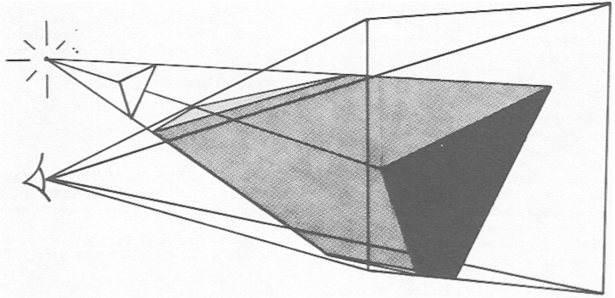
\includegraphics[width=0.9\linewidth]{fig4}
\caption[fig4]{按视场裁剪的阴影多边形}
\label{fig:fig4}
\end{figure*}
必须保持这个多边形的辨识,这样一个阴影体积(正面多边形)的近表面才能从远表面(背面多边形)中区分出来。
所以面向光源的多边形,加上一个物体的投射阴影多边形的集合,共同确定了该物体的阴影体积。\\
当应用一个扫描隐藏表面算法时,阴影多边形可以就像其他数据那样处理。
只有可见表面的阴影才需要不同的处理方式。
阴影多边形本身是不可见的,所以它们不用计入可见性的决定中。
但是,阴影表面的深度顺序和可见的表面决定了阴影。
一个正面阴影表面使任何之后的东西置于阴影中,而一个背面阴影表面取消了正面阴影表面的效果。
例如,一个桩子或者柱子可能投射一个包含单个多边形对的的阴影表面。
任何在这两个阴影多边形间的表面都会在阴影中,而在这两个多边形前面或者后面的表面则是正常地被遮盖。\\
如果最前面的阴影表面是背面的,那么任何在它前面的东西都在阴影中。
如果最后面的阴影表面是正面的,那么任何在它后面的东西都在阴影中。
当出射点在阴影中,或者表面在视场的很大一部分上投射了阴影了,这种情况就会出现。
所以,无论何时,只要表面在一个背面的最前阴影多边形之前,或者这个表面刺透的正面阴影多边形比背面阴影多边形多,那这个表面就在阴影中。
在一个可见表面和一个阴影多边形相交的地方,就会形成阴影边界。\\
为了处理阴影多边形,要对扫描隐藏表面算法进行调整,包含仅改变计算阴影的内循环。
可以用阴影多边形的两个性质来简化计算。
第一,阴影多边形是不可见的。
所以,只包含阴影多边形的扫描线可以被忽略。
第二,由轮廓边投影形成的阴影多边形不会和另一个相交(只要用的是单个光源)。
所以这些多边形的深度顺序是不变的。\\
使用Bouknight的扫描算法的变种(这种类型算法的详细描述可见\cite{4}\cite{12}),在y方向排序,x方面合并的步骤中,阴影多边形可以像其他多边形那样处理。
通常,扫描算法需要维护一个按深度排序的所有被扫描片段的列表,这些片段在扫描线上会被一束由当前位置出射点射出的光线穿透。
阴影多边形会频繁地导致相当长的扫描片段,大大地增加了一张图像的平均深度复杂度。
正如Sutherland等人\cite{12}指出的,深度复杂度的增加会严重阻碍扫描算法的表现。\\
但是,在产生扫描片段期间,阴影多边形只需在某些条件下考虑。
阴影多边形不会相交的事实允许有利地利用扫描线到扫描线的一致性。
随着扫描向图像下方移动,只有当新的多边形添加进来,或者旧的多边形被删除时,阴影多边形的深度顺序才会改变。
所以重建和更新阴影多边形的深度序列的过程可以极大地缩减。
只有当物体片段出现时,这个列表才需要构建。
所以,一条没有任何物体片段的扫描线可以被忽略。
因为深度顺序不会改变,所以只有当一个阴影表面需要和一个可见表面比较深度顺序时,才有必要计算这个阴影表面的深度。\\
只有当图像的可见表面改变时,才需要搜索阴影多边形的优先级列表。
一旦发现了哪个阴影多边形和现在的可见表面(在深度上)绑定了,那么只有这些多边形需要为了可能的相交作检查。
所以,尽管可能会因为阴影而有相当大的深度复杂性,也就差不多两到三个阴影表面的深度复杂度会真的影响计算时间。
但是,现在许多图像平均有少于三个的深度复杂度。
因此,增加阴影多边形数量,会导致扫描过程需要的时间的显著增加。
不过,在尝试更高复杂度的环境中,这种影响被证实为没那么重要。
	\section{三类方法间的比较}
关于在使用上述方法表示阴影时的附加困难,我们可以做个比较。
我们使用三个比较标准:
需要的额外数据存储空间,
需要的额外计算量,
所需的额外软件的实现难易。
在判定的时候,我们假设用扫描隐藏表面算法。\\
初看一眼,只有第二类和第三类算法看起来需要额外的数据存储。
两遍的方法要求表面沿着阴影边界分开,或者至少要在数据中包含阴影边界。
阴影多边形的方法要求存储可能的大量阴影多边形。
但是,这两类算法都不要求整个场景描述,用来进行隐藏表面计算。
背面表面和视场之外的数据可以被丢弃。
另一方面,第一类算法要求所有物体一直以原始数据的方式呈现,这样投影阴影边界才能在扫描期间计算出来。
所以,留给隐藏表面算法的后续步骤所需的临时空间就会严重缩减。
一定可以得出的结论是:两遍的方式需要最少的额外存储空间,阴影多边形的方式需要稍多一些的空间,而扫描时计算阴影的方式需要最多的空间。\\
假设仅使用外围来计算阴影边界总是更高效的,那么投射阴影多边形的方式似乎产生的必要计算的增加的是最少的。
一旦找到了外围边,那么阴影多边形的定义是很直观的。
通过利用阴影多边形的特殊性质,在扫描期间要做的额外计算量是最少的。
更进一步,另外两种方式要求方法遵循更低要求的增长律。
在扫描时计算阴影的方式要求额外的计算量,这是为了决定哪些表面可能投射阴影到其他表面上。并且通过操作物体空间数据,要求计算分割开有阴影区域和无阴影区域的线段。
Bouknight和Kelley概略地汇报说每次单个场景的阴影计算会扩大两倍的计算量。
反之,两遍的方式要求对于隐藏表面算法的额外解决方案。
但是,因为只要考虑外围边,第一遍可以简化。\\
对于投射阴影多边形的方式而言,所需的额外软件的复杂度同样是最低的。
第一类和第二类算法都要求完全新的软件。
不过,可以说,一旦一个合适的,针对于两遍的方式的隐藏表面算法出现了,那么第一遍所需的软件仅仅是第二遍所需软件的子集,所以并不需要额外的软件。\\
给定一个有可用扫描隐藏表面算法的情景,看起来阴影多边形的方式提供了最佳解决方案。
不过,从头开始的话,并没有一个清晰的最佳选择。
当然,通过实现任何一类的算法,也可以学到很多东西。
	\section{鸣谢}
这里表述的大部分想法源自于和Utah大学同事的交流。
尤其是Ivan Sutherland建议我关注投射阴影多边形的概念,还提供了很多对这篇论文初稿的有用的建议。
	
	%----------------------------------------------------------------------------------------
	%	REFERENCE LIST
	%----------------------------------------------------------------------------------------
	\renewcommand{\refname}{参考文献}
	\begin{thebibliography}{99} % Bibliography - this is intentionally simple in this template
		
		\bibitem{1}
		Appel, A.,
		\newblock {\em The Notion of Quantitative Invisibility and the Machine Rendering of Solids, } 
		\newblock Proceedings ACM 1967 National Conference.
		
		\bibitem{2}
		Appel, A.,
		\newblock {\em Some Techniques for Shading Machine Renderings of Solids, } 
		\newblock 1968 SJCC, AFIPS Vol. 32.
		
		\bibitem{3}
		Appel, A.,
		\newblock {\em On Calculating the Illusion of Reality, } 
		\newblock IFIP 1968.
		
		\bibitem{4}
		Bouknight, W. J.,
		\newblock {\em A Procedure for the Generation of 3-D Half-Toned Computer Graphics Presentations,} 
		\newblock CACM, Vol. 13, no. 6, Sept. 1970.
		
		\bibitem{5}
		Bouknight, W. J. and Kelley, K.,
		\newblock {\em An Algorithm for Producing Half-Tone Computer Graphics Presentations with Shadows and Moveable Light Sources,} 
		\newblock 1970 SJCC, AFIPS Vol. 36.
		
		\bibitem{6}
		Bui Tuong Phong and Crow, F. C.,
		\newblock {\em Improved Rendition of Polygonal Models of Curved Surfaces,} 
		\newblock Proc. of the 2nd USA-Japan Computer Conf., 1975.
		
		\bibitem{7}
		Clark, J. H.,
		\newblock {\em Hierarchical Geometric Models for Visible Surface Algorithms,} 
		\newblock CACM, Vol. 19 no. 10, Oct. 1976.
		
		\bibitem{8}
		Crow, F. C.,
		\newblock {\em The Aliasing Problem in Computer- Synthesized Shaded Images,} 
		\newblock Dept of Computer Science University of Utah, UTEC-CSc-76-015, March 1976. (abridged version to appear in CACM)
		
		\bibitem{9}
		Newell, M. G., Newell, R. G. and Sancha, T. L.
		\newblock {\em A Solution to the Hidden-Surface Problem,} 
		\newblock Proceedings of the 1972 ACM National Conference.
		
		\bibitem{10}
		Newell, M. G.,
		\newblock {\em The Utilization of Procedural Models in Digital Image Synthesis,} 
		\newblock Department of Computer Science, University of Utah, UTEC-CSc-76-218, Summer 1975.
		
		\bibitem{11}
		Sutherland, I. E.,
		\newblock {\em Polygon Sorting by Subdivision: A Solution to the Hidden-Surface Problem,} 
		\newblock Unpublished, 1973.
		
		\bibitem{12}
		Sutherland, I. E., Sproull, R. F. and Schu- maker, R. G.,
		\newblock {\em A Characterization of Ten Hidden- Surface Algorithms,} 
		\newblock Computing Surveys, Vol. 6, No. 1, March 1974.
		
\end{thebibliography}
	
	%----------------------------------------------------------------------------------------
\end{CJK}	
\end{document}
